% Options for packages loaded elsewhere
% Options for packages loaded elsewhere
\PassOptionsToPackage{unicode}{hyperref}
\PassOptionsToPackage{hyphens}{url}
\PassOptionsToPackage{dvipsnames,svgnames,x11names}{xcolor}
%
\documentclass[
  french,
  11pt,
  a4paper,
  oneside]{report}
\usepackage{xcolor}
\usepackage[top=1.5cm, bottom=1.5cm, left=2.5cm, right=2.5cm]{geometry}
\usepackage{amsmath,amssymb}
\setcounter{secnumdepth}{-\maxdimen} % remove section numbering
\usepackage{iftex}
\ifPDFTeX
  \usepackage[T1]{fontenc}
  \usepackage[utf8]{inputenc}
  \usepackage{textcomp} % provide euro and other symbols
\else % if luatex or xetex
  \usepackage{unicode-math} % this also loads fontspec
  \defaultfontfeatures{Scale=MatchLowercase}
  \defaultfontfeatures[\rmfamily]{Ligatures=TeX,Scale=1}
\fi
\usepackage{lmodern}
\ifPDFTeX\else
  % xetex/luatex font selection
\fi
% Use upquote if available, for straight quotes in verbatim environments
\IfFileExists{upquote.sty}{\usepackage{upquote}}{}
\IfFileExists{microtype.sty}{% use microtype if available
  \usepackage[]{microtype}
  \UseMicrotypeSet[protrusion]{basicmath} % disable protrusion for tt fonts
}{}
\makeatletter
\@ifundefined{KOMAClassName}{% if non-KOMA class
  \IfFileExists{parskip.sty}{%
    \usepackage{parskip}
  }{% else
    \setlength{\parindent}{0pt}
    \setlength{\parskip}{6pt plus 2pt minus 1pt}}
}{% if KOMA class
  \KOMAoptions{parskip=half}}
\makeatother
% Make \paragraph and \subparagraph free-standing
\makeatletter
\ifx\paragraph\undefined\else
  \let\oldparagraph\paragraph
  \renewcommand{\paragraph}{
    \@ifstar
      \xxxParagraphStar
      \xxxParagraphNoStar
  }
  \newcommand{\xxxParagraphStar}[1]{\oldparagraph*{#1}\mbox{}}
  \newcommand{\xxxParagraphNoStar}[1]{\oldparagraph{#1}\mbox{}}
\fi
\ifx\subparagraph\undefined\else
  \let\oldsubparagraph\subparagraph
  \renewcommand{\subparagraph}{
    \@ifstar
      \xxxSubParagraphStar
      \xxxSubParagraphNoStar
  }
  \newcommand{\xxxSubParagraphStar}[1]{\oldsubparagraph*{#1}\mbox{}}
  \newcommand{\xxxSubParagraphNoStar}[1]{\oldsubparagraph{#1}\mbox{}}
\fi
\makeatother

\usepackage{color}
\usepackage{fancyvrb}
\newcommand{\VerbBar}{|}
\newcommand{\VERB}{\Verb[commandchars=\\\{\}]}
\DefineVerbatimEnvironment{Highlighting}{Verbatim}{commandchars=\\\{\}}
% Add ',fontsize=\small' for more characters per line
\usepackage{framed}
\definecolor{shadecolor}{RGB}{241,243,245}
\newenvironment{Shaded}{\begin{snugshade}}{\end{snugshade}}
\newcommand{\AlertTok}[1]{\textcolor[rgb]{0.68,0.00,0.00}{#1}}
\newcommand{\AnnotationTok}[1]{\textcolor[rgb]{0.37,0.37,0.37}{#1}}
\newcommand{\AttributeTok}[1]{\textcolor[rgb]{0.40,0.45,0.13}{#1}}
\newcommand{\BaseNTok}[1]{\textcolor[rgb]{0.68,0.00,0.00}{#1}}
\newcommand{\BuiltInTok}[1]{\textcolor[rgb]{0.00,0.23,0.31}{#1}}
\newcommand{\CharTok}[1]{\textcolor[rgb]{0.13,0.47,0.30}{#1}}
\newcommand{\CommentTok}[1]{\textcolor[rgb]{0.37,0.37,0.37}{#1}}
\newcommand{\CommentVarTok}[1]{\textcolor[rgb]{0.37,0.37,0.37}{\textit{#1}}}
\newcommand{\ConstantTok}[1]{\textcolor[rgb]{0.56,0.35,0.01}{#1}}
\newcommand{\ControlFlowTok}[1]{\textcolor[rgb]{0.00,0.23,0.31}{\textbf{#1}}}
\newcommand{\DataTypeTok}[1]{\textcolor[rgb]{0.68,0.00,0.00}{#1}}
\newcommand{\DecValTok}[1]{\textcolor[rgb]{0.68,0.00,0.00}{#1}}
\newcommand{\DocumentationTok}[1]{\textcolor[rgb]{0.37,0.37,0.37}{\textit{#1}}}
\newcommand{\ErrorTok}[1]{\textcolor[rgb]{0.68,0.00,0.00}{#1}}
\newcommand{\ExtensionTok}[1]{\textcolor[rgb]{0.00,0.23,0.31}{#1}}
\newcommand{\FloatTok}[1]{\textcolor[rgb]{0.68,0.00,0.00}{#1}}
\newcommand{\FunctionTok}[1]{\textcolor[rgb]{0.28,0.35,0.67}{#1}}
\newcommand{\ImportTok}[1]{\textcolor[rgb]{0.00,0.46,0.62}{#1}}
\newcommand{\InformationTok}[1]{\textcolor[rgb]{0.37,0.37,0.37}{#1}}
\newcommand{\KeywordTok}[1]{\textcolor[rgb]{0.00,0.23,0.31}{\textbf{#1}}}
\newcommand{\NormalTok}[1]{\textcolor[rgb]{0.00,0.23,0.31}{#1}}
\newcommand{\OperatorTok}[1]{\textcolor[rgb]{0.37,0.37,0.37}{#1}}
\newcommand{\OtherTok}[1]{\textcolor[rgb]{0.00,0.23,0.31}{#1}}
\newcommand{\PreprocessorTok}[1]{\textcolor[rgb]{0.68,0.00,0.00}{#1}}
\newcommand{\RegionMarkerTok}[1]{\textcolor[rgb]{0.00,0.23,0.31}{#1}}
\newcommand{\SpecialCharTok}[1]{\textcolor[rgb]{0.37,0.37,0.37}{#1}}
\newcommand{\SpecialStringTok}[1]{\textcolor[rgb]{0.13,0.47,0.30}{#1}}
\newcommand{\StringTok}[1]{\textcolor[rgb]{0.13,0.47,0.30}{#1}}
\newcommand{\VariableTok}[1]{\textcolor[rgb]{0.07,0.07,0.07}{#1}}
\newcommand{\VerbatimStringTok}[1]{\textcolor[rgb]{0.13,0.47,0.30}{#1}}
\newcommand{\WarningTok}[1]{\textcolor[rgb]{0.37,0.37,0.37}{\textit{#1}}}

\usepackage{longtable,booktabs,array}
\usepackage{calc} % for calculating minipage widths
% Correct order of tables after \paragraph or \subparagraph
\usepackage{etoolbox}
\makeatletter
\patchcmd\longtable{\par}{\if@noskipsec\mbox{}\fi\par}{}{}
\makeatother
% Allow footnotes in longtable head/foot
\IfFileExists{footnotehyper.sty}{\usepackage{footnotehyper}}{\usepackage{footnote}}
\makesavenoteenv{longtable}
\usepackage{graphicx}
\makeatletter
\newsavebox\pandoc@box
\newcommand*\pandocbounded[1]{% scales image to fit in text height/width
  \sbox\pandoc@box{#1}%
  \Gscale@div\@tempa{\textheight}{\dimexpr\ht\pandoc@box+\dp\pandoc@box\relax}%
  \Gscale@div\@tempb{\linewidth}{\wd\pandoc@box}%
  \ifdim\@tempb\p@<\@tempa\p@\let\@tempa\@tempb\fi% select the smaller of both
  \ifdim\@tempa\p@<\p@\scalebox{\@tempa}{\usebox\pandoc@box}%
  \else\usebox{\pandoc@box}%
  \fi%
}
% Set default figure placement to htbp
\def\fps@figure{htbp}
\makeatother



\ifLuaTeX
\usepackage[bidi=basic]{babel}
\else
\usepackage[bidi=default]{babel}
\fi
% get rid of language-specific shorthands (see #6817):
\let\LanguageShortHands\languageshorthands
\def\languageshorthands#1{}


\setlength{\emergencystretch}{3em} % prevent overfull lines

\providecommand{\tightlist}{%
  \setlength{\itemsep}{0pt}\setlength{\parskip}{0pt}}



 


\usepackage{graphicx}
\usepackage{fancyhdr}

\pagestyle{fancy}
\fancyhf{}

\fancyfoot[C]{\thepage}

\fancyhead[R]{\raisebox{-0.3cm}{
\includegraphics[width=2cm]{Images/ensai_logo_1.png}}}

\renewcommand{\headrulewidth}{0pt}
\renewcommand{\footrulewidth}{0pt}

\fancypagestyle{plain}{
  \fancyhf{}
  \fancyfoot[C]{\thepage}
  \fancyhead[R]{\raisebox{-0.3cm}{
\includegraphics[width=2cm]{Images/ensai_logo_1.png}}}
  \renewcommand{\headrulewidth}{0pt}
\makeatletter
\@ifpackageloaded{tcolorbox}{}{\usepackage[skins,breakable]{tcolorbox}}
\@ifpackageloaded{fontawesome5}{}{\usepackage{fontawesome5}}
\definecolor{quarto-callout-color}{HTML}{909090}
\definecolor{quarto-callout-note-color}{HTML}{0758E5}
\definecolor{quarto-callout-important-color}{HTML}{CC1914}
\definecolor{quarto-callout-warning-color}{HTML}{EB9113}
\definecolor{quarto-callout-tip-color}{HTML}{00A047}
\definecolor{quarto-callout-caution-color}{HTML}{FC5300}
\definecolor{quarto-callout-color-frame}{HTML}{acacac}
\definecolor{quarto-callout-note-color-frame}{HTML}{4582ec}
\definecolor{quarto-callout-important-color-frame}{HTML}{d9534f}
\definecolor{quarto-callout-warning-color-frame}{HTML}{f0ad4e}
\definecolor{quarto-callout-tip-color-frame}{HTML}{02b875}
\definecolor{quarto-callout-caution-color-frame}{HTML}{fd7e14}
\makeatother
\makeatletter
\@ifpackageloaded{caption}{}{\usepackage{caption}}
\AtBeginDocument{%
\ifdefined\contentsname
  \renewcommand*\contentsname{Table des matières}
\else
  \newcommand\contentsname{Table des matières}
\fi
\ifdefined\listfigurename
  \renewcommand*\listfigurename{Liste des Figures}
\else
  \newcommand\listfigurename{Liste des Figures}
\fi
\ifdefined\listtablename
  \renewcommand*\listtablename{Liste des Tables}
\else
  \newcommand\listtablename{Liste des Tables}
\fi
\ifdefined\figurename
  \renewcommand*\figurename{Figure}
\else
  \newcommand\figurename{Figure}
\fi
\ifdefined\tablename
  \renewcommand*\tablename{Table}
\else
  \newcommand\tablename{Table}
\fi
}
\@ifpackageloaded{float}{}{\usepackage{float}}
\floatstyle{ruled}
\@ifundefined{c@chapter}{\newfloat{codelisting}{h}{lop}}{\newfloat{codelisting}{h}{lop}[chapter]}
\floatname{codelisting}{Listing}
\newcommand*\listoflistings{\listof{codelisting}{Liste des Listings}}
\makeatother
\makeatletter
\makeatother
\makeatletter
\@ifpackageloaded{caption}{}{\usepackage{caption}}
\@ifpackageloaded{subcaption}{}{\usepackage{subcaption}}
\makeatother
\usepackage{bookmark}
\IfFileExists{xurl.sty}{\usepackage{xurl}}{} % add URL line breaks if available
\urlstyle{same}
\hypersetup{
  pdftitle={Relation élèves enseignants},
  pdfauthor={Barbeau Faustine - Combes Florent - Dumas Elouan - Malzieu Yann},
  pdflang={fr},
  colorlinks=true,
  linkcolor={blue},
  filecolor={Maroon},
  citecolor={Blue},
  urlcolor={Blue},
  pdfcreator={LaTeX via pandoc}}


\title{Relation élèves enseignants}
\author{Barbeau Faustine - Combes Florent - Dumas Elouan - Malzieu Yann}
\date{}
\begin{document}
\maketitle

\renewcommand*\contentsname{Table des matières}
{
\hypersetup{linkcolor=}
\setcounter{tocdepth}{2}
\tableofcontents
}

\renewcommand{\contentsname}{Table des matières}

\chapter{Introduction}\label{introduction}

``La relation élève-enseignant s'intéresse à ce qui se passe entre
l'enseignant et ses élèves, à l'école, d'un point de vue à la fois
cognitif, affectif et social, au-delà des savoirs scolaires'' (Espinosa,
2016). Selon lui, l'enseignement constitue un facteur à part entière de
l'éducation des élèves, car même si cette dernière relève
majoritairement de la responsabilité des parents, l'impact des
professeurs dans la vie des élèves reste non negligeable. Ainsi, cette
affirmation s'observe-t-elle réellement dans la réalité ? La relation
entre les élèves et leurs enseignants ne se limite-t-elle pas uniquement
à un cadre scolaire ? Une bonne relation élève/enseignant
implique-t-elle la performance académique de l'élève ? Toutes ces
interrogations nous amènent à nous intéresser au sujet suivant : La
relation entre élèves et enseignants (REE).

La relation élèves enseignants caractérise une intéraction, qu'elle soit
poisitive ou négative, entretenue entre les élèves et les enseignants.
Cette relation s'inscrit dans une dynamique de transmission des savoirs
et peut être qualifiée de verticale, dans la mesure où l'enseignant
détient un savoir que l'élève est en train d'acquérir. Elle possède
également une dimension subjective, puisqu'elle repose en grande partie
sur le ressenti des élèves. Ainsi sa meusre repose nécessairement sur
des données déclarative, susceptible de comporter certain biais.

Dans notre étude nous allons donc mesurer cette REE, et nous nous
demanderons si une bonne relation entre élèves et enseignants influence
positivement la scolarité des élèves à différentes échelles.

Dans un premier temps, il s'agira de comprendre ce qu'est la relation
élèves-enseignants à travers la manière dont elle est perçue par les
élèves, ainsi que d'analyser les cas de non-réponse. Ensuite, nous
étudierons les liens entre la REE et la réussite scolaire, en tenant
compte des performances individuelles, des différences entre pays et du
contexte socio-économique. Enfin, nous nous intéresserons aux relations
entre la REE et le bien-être des élèves dans le cadre scolaire,
notamment en termes d'anxiété et de relations entre pairs.

Les données utilisées sont issues de l'enquête PISA 2022, qui interroge
des élèves âgés de 15 habitant dans 85 pays. Cette base de données
permet d'accéder à des informations portant sur les performances
scolaires, le contexte socio-économique des élèves, leur ressenti
vis-à-vis de l'école ainsi que leur relation avec leurs enseignants.

\chapter{1 Une étude de la relation élèves-enseignants limitée par les
non-réponses}\label{une-uxe9tude-de-la-relation-uxe9luxe8ves-enseignants-limituxe9e-par-les-non-ruxe9ponses}

\section{1.1 Cadre d'analyse de la REE}\label{cadre-danalyse-de-la-ree}

En premier lieu, afin de définir le cadre dans lequel nous nous plaçons,
il faut avant tout préciser comment se caractérisent élèves et
enseignants dans le questionnaire PISA. En effet, pour un élève, il
s'agit ici d'un enfant âgé d'environ 15 ans unscrut dans un
établissement scolaire public, privé ou bien spécialisé et pouvant
provenir de 85 pays différents pour l'édition 2022. Par ailleurs, les
enseignants sont, par définition, les professeurs des élèves interrogés
dans l'enquête PISA.

Ainsi, nous nous plaçons dans un contexte particulier d'analyse
puisqu'il faut dan notre cas, étudier la REE grâce aux données présentes
sur les questionnaire PISA 2022. Cette base de données permet d'accéder
à des informations portant sur les performances scolaires, le contexte
socio-économiques des élèves, leur ressenti vis-à-vis de l'école ainsi
que leur relation avec leurs enseignants. C'est pourquoi, afin de
pouvoir réaliser notre étude, il nous fallait proposer une mesure des
différents types de REE sur lesquels nous souhaitons nous appuyer.
Ainsi, nous avons utilise deux indices déjà créés par l'OCDE afin de
caractérier cette relation. En particulier, nous avons choisi de
travailler avec l'indice mesurant la REE globale (RELATST), qui comprend
des questions générales sur le ressenti de l'élève quant à ses
interactions avec leur enseignants, mais également l'indice mesurant la
REE ciblée sur les professeurs de mathématiques(TEACHSUP) (voir annexe
pour la construction des indices).

Toutefois, une potentielle limite de notre analyse mais inhérente au
questionnaire PISA, est qu'il ne prend en compte la REE dans un seul
sens. En effet, dans la réalité, les enseignants ont une influence sur
leurs élèves mais l'inverse est aussi véridique, les élèves peuvent
modifier le comportement de leurs professeurs. Cependant, ce deuxième
sens dans la REE ne peut être vérifiée dans cette enquête, car seuls les
élèves expriment leur opinion sur leurs professeurs.

\section{1.2 L'absence de certains pays dans l'étude de la
REE}\label{labsence-de-certains-pays-dans-luxe9tude-de-la-ree}

Une solution simple permettant de faire les anaylses est d'imputer les
valeurs manquantes par la moyenne. Cependant lorsqu'on regarde en détail
ces non réponses on retrouve quelques informations très importantes.

L'enquête PISA se base sur un questionnaire distribuée par les pays dans
les écoles, cependant chaque partie du questionnaire étant facultative,
un pays a pu refuser sa distribution pour certaines raisons. Pour
l'indice mesurant la relation entre élèves et enseignant dans la
globalité on retrouve de nombreux pays avec un taux de non-réponses égal
à 100\%. Les pays sont Brunei, Canada, Indonésie, Israël, Cambodge,
Macao, Maroc, Malaisie, Philippines et Ouzbékistan. Cependant d'après
nos recherches aucune raison officielle ne permet de conclure sur la
raison de la non distribution de cette partie du questionnaire.

Il serait donc non approprié d'amputer seulement toutes les non-réponses
par la moyenne totale pour les pays n'ayant pas distribués cette partie
du questionnaire correspondant à la construction de l'indice. Nous
allons donc supprimés ces pays de notre jeu de données.

\pandocbounded{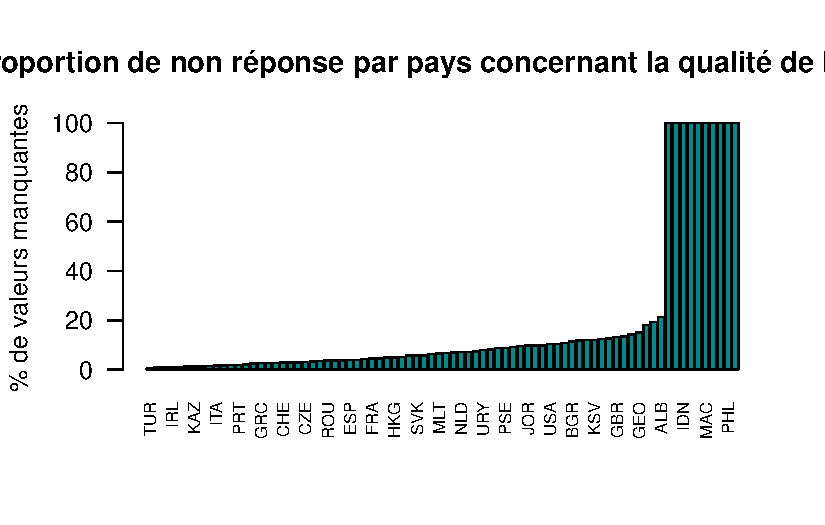
\includegraphics[keepaspectratio]{brouillon_rapport_files/figure-pdf/unnamed-chunk-8-1.pdf}}

Figure 2: Illustration du taux de non-réponses pour l'indice de relation
entre élèves et enseignants. Note de lecture : Le Brunei a un taux de
non réponse de 100\% sur les données concernant l'indice de qualité de
la relation entre élèves et enseignants.

\section{1.3 Les profils des élèves qui ne se positionnent pas sur leur
relation avec le corps
enseignant}\label{les-profils-des-uxe9luxe8ves-qui-ne-se-positionnent-pas-sur-leur-relation-avec-le-corps-enseignant}

Maintenant que nos données sont nettoyés, nous pouvons faire une analyse
du profil des élèves qui n'ont pas répondu aux questions sur leur
relation avec le corps enseignant. En premier lieu nous voyons que dans
la figure 3, il existe une relation entre le fait de ne pas avoir
d'incide de REE et la moyenne générale. Ne pas avoir d'incide de REE
signifie ne pas avoir répondu à toutes les questions qui servent à
construire de celui-ci. En effet on remarque que la distribution de la
moyenne générale des élèves n'ayant pas d'indice de REE est plus centrée
sur la gauche que la distribution pour les élèves ayant un indice de
REE. On peut donc en conclure que les élèves qui ne se positionnement
pas sur leur relation avec le corps enseignants sont des élèves avec une
moyenne générale plus faible que ceux se positionnant.

\pandocbounded{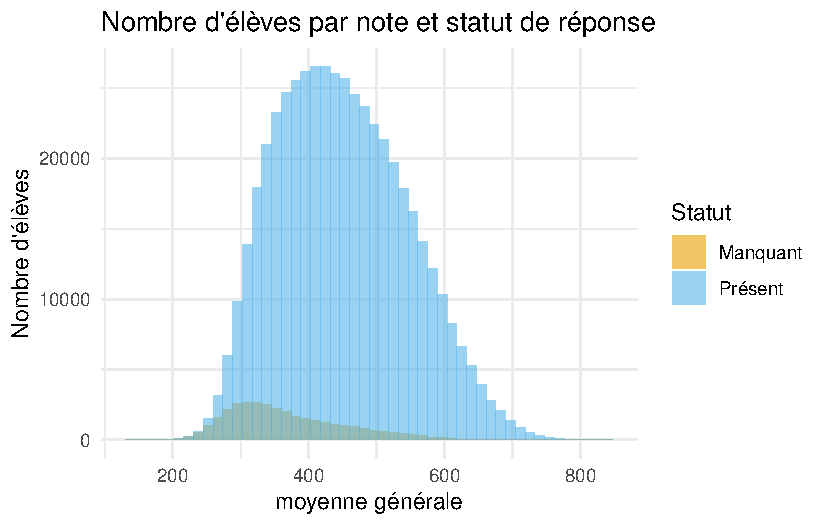
\includegraphics[keepaspectratio]{brouillon_rapport_files/figure-pdf/unnamed-chunk-11-1.pdf}}

Figure 3: Graphique indiquant la distribution de la moyenne générale en
fonction de la présence d'un indice de REE ou non. Note de lecture : La
distribution de la moyenne générale des élèves n'ayant pas d'indice de
REE est plus centrée sur la gauche que la distribution pour les élèves
ayant un indice de REE.

Concernant les autres variables nous pouvons analyser grâce aux tableau
1, que les élèves n'ayant pas d'indice REE sont du genre plutôt
masculin. En effet on retrouve 38.2\% de femmes pour un indice REE
manquant quand celui-ci est à 49.7\% pour l'ensemble des données.

\begin{verbatim}
# A tibble: 2 x 7
  Groupe   Pourcentage_filles Origine_socioeco Anxiete_maths Appartenance
  <chr>                 <dbl>            <dbl>         <dbl>        <dbl>
1 Manquant               38.2           -0.776         0.381      -0.214 
2 Ensemble               49.7           -0.250         0.225      -0.0590
# i 2 more variables: Harcelement <dbl>, Nombre_total <int>
\end{verbatim}

Table 1: Comparaison entre les élèves ayant un indice REE et ceux n'en
ayant pas Note de lecture: Pour les élèves n'ayant pas d'indice REE ils
ont une moyenne d'indice d'anxiété par rapport aux mathématiques de
0.381.

\section{1.4 Une relation décrite comme globalement
positive}\label{une-relation-duxe9crite-comme-globalement-positive}

Il est maintenant intéressant de s'interresser à la qualité de cette
relation et savoir comment elle est perçue par les élèves. Car un indice
relève en effet de la qualité au global de la relation mais il est aussi
immportant de savoir le détail par question. Pour cela nous avons
récupéré le taux de réponse positives par question en ce qui concerne la
relation élève-enseignant au global et celle sur les professeurs de
mathématiques, seulement pour les élèves ayant répondu à la question. On
remarque que les résultats sont très positives, la question ayant le
moins bon résultat est ``Les enseignants font attention aux élèves en
cas de retard'', avec 72,7\% de réponses positives. Donc pour seulement
27.3\% les élèves l'enseignant ne fait pas attention. Quand aux autres
résultats, ils se situent entre 79.4\% et 94.2\% de réponses positives
donc seulement 20.6\% et 4.8\% de réponses négatives. On peut conclure
que les trois qualités qui caratérisent au mieux cette relation positive
sont un enseignant qui n'est pas méchant, qui est amical et qui se
soucit du bien-être des élèves.

\pandocbounded{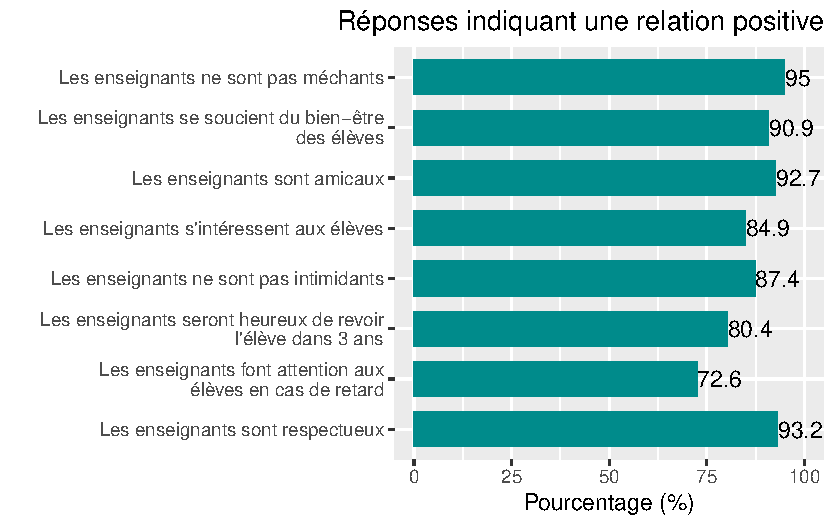
\includegraphics[keepaspectratio]{brouillon_rapport_files/figure-pdf/unnamed-chunk-14-1.pdf}}

Figure 1: Illustration du taux de réponses positives par question Note
de lecture : 85\% des élèves ayant répondu affirment que leurs
enseignants sont respectueux envers eux.

Cette relation étant très positive en ce qui concerne les enseignant au
global, maintenant interessons nous aux enseignants de mathèmatiques. On
a donc sur la figure suivant le taux de réponse positive pour les
questions concernant les enseignants de mathématiques. Les résultats
sont très différents de ce qu'on a pu observer avec les enseignants dans
leur globalité. En effet les taux de réponses positives se trouve
seulement entre 25.4\% et 32.2\%, on se retrouve donc avec une majorité
de réponses négatives contrairement à la relation globale.

\pandocbounded{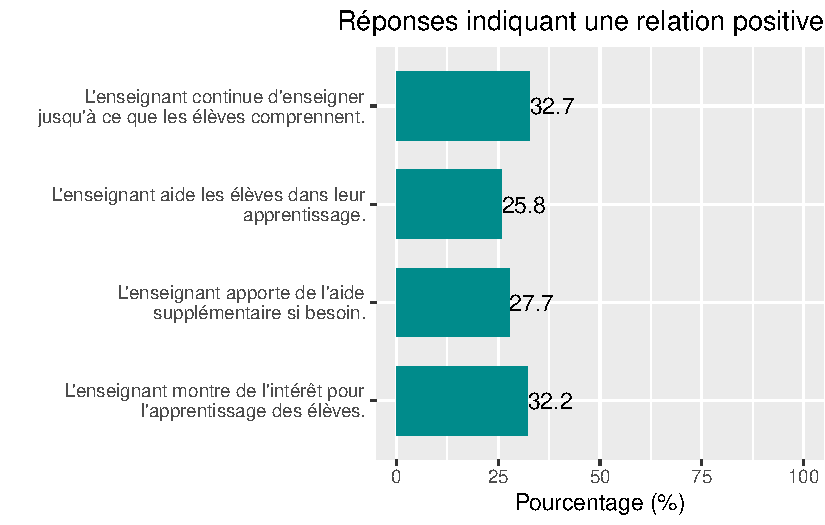
\includegraphics[keepaspectratio]{brouillon_rapport_files/figure-pdf/unnamed-chunk-15-1.pdf}}

Figure 2: Illustration du taux de réponses positives par question
concernant les professeurs de mathématiques Note de lecture : 32.2\% des
élèves ayant répondu affirment que leur enseignant montre de l'intérêt
pour l'apprentissage des éléves.

Cependant, nous avons affichés les résultats seulement pour les élèves
ayant répondu aux questions. Si l'on regarde le taux de non réponses
nous avons 43.04\% de non réponses concernant la relations dans la
globalité et 15.53\% pour la relation avec les professeurs de
mathématiques. Le chiffre de non-réponse nous poussent à s'interroger
sur le profil des élèves qui ne répondent pas pour comprendre en quoi
cela pourrait biaiser nos analyses futures.

\chapter{2 La REE et la réussite scolaire : une relation
complexe}\label{la-ree-et-la-ruxe9ussite-scolaire-une-relation-complexe}

\section{2.1 Relation entre REE et niveau académique
individuel}\label{relation-entre-ree-et-niveau-acaduxe9mique-individuel}

La relation élèves-enseignant peut être étudiée dans le cadre de la
réussite scolaire et plus précisemment concernant le niveau académique
des élèves. Comme la REE est une relation prenant place au sein des
établissements scolaires, il est tout à fait naturel de s'interroger sur
l'influence de la REE sur le niveau des élèves et inversement. Le niveau
scolaire est ici étudié au travers des notes établies par l'OCDE lors de
l'enquête PISA 2022. Celle-ci permettent de connaître le niveau relatif
des élèves concernant différents domaines d'études. Pour comprendre au
mieux la relation que le niveau scolaire peut entretenir avec la REE,
les analyses vont se porter sur la moyenne générale obtenue par les
élèves ainsi que la moyenne de mathématiques.

\pandocbounded{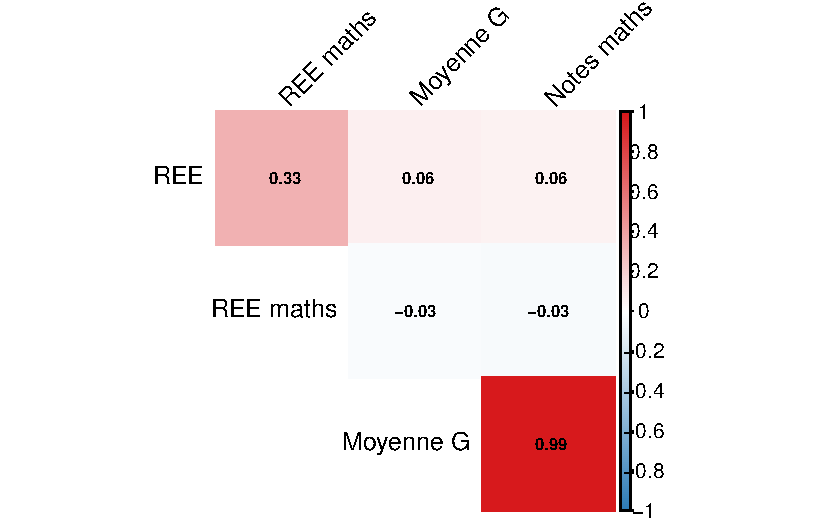
\includegraphics[keepaspectratio]{brouillon_rapport_files/figure-pdf/unnamed-chunk-17-1.pdf}}

Note de lecture : La corrélation entre la relation élèves-enseignants
(REE) et la moyenne générale est de 0.06.

Ainsi, contrairement à ce que l'on peut penser a priori, le niveau
académique des élèves n'explique pas la qualité de la relation avec
leurs enseignants. Le lien de corrélation est presque nul (0.06). Par
conséquent, un élève peut potentiellement bien s'entendre avec son
professeur sans pour autant que cela ait une influence sur ses résultats
scolaires. D'autres facteurs semblent donc être à la source de la
réussite scolaire des élèves qu'une bonne relation entre élève et
enseignant au niveau global.

\section{2.2 Relation entre REE et niveau académique
national}\label{relation-entre-ree-et-niveau-acaduxe9mique-national}

Comme on constate qu'il n'y a pas de lien entre REE et notes pour les
élèves, on peut aussi étudier cette relation à l'échelle des pays. Dans
cette analyse, on utilise la moyenne de REE dans chaque pays et la
moyenne des notes obtenues. Cela permet de comparer les niveau nationaux
et donc de comparer les différents systèmes éducatifs et leurs
influences sur la REE.

Il existe une corrélation négative très faible entre la qualité de la
REE et la note moyenne de chaque pays (r =\textasciitilde{} -0,26). La
REE n'explique que partiellement le niveau académique mais d'autres
facteurs entre en compte. On ne peut donc pas conclure d'une relation
très forte entre ces deux indicateurs.

En se concentrant sur la REE avec les enseignants de mathématiques, on
observe des résultats plus marqués. La note moyenne utilisée est
désormais celle des mathématiques et non plus la moyenne générale.

Plus un pays dispose d'un niveau en mathématiques élevé selon les notes
de l'OCDE, moins la relation entre les élèves et les enseignants de
mathématiques est jugée positive. En effet, on constate une corrélation
négative (r =\textasciitilde{} -0.51, p-value =\textasciitilde{} 5e-06)
entre la qualité de la REE moyenne d'un pays et sa note OCDE moyenne
concernant les mathématiques.

\begin{verbatim}
`geom_smooth()` using formula = 'y ~ x'
\end{verbatim}

\pandocbounded{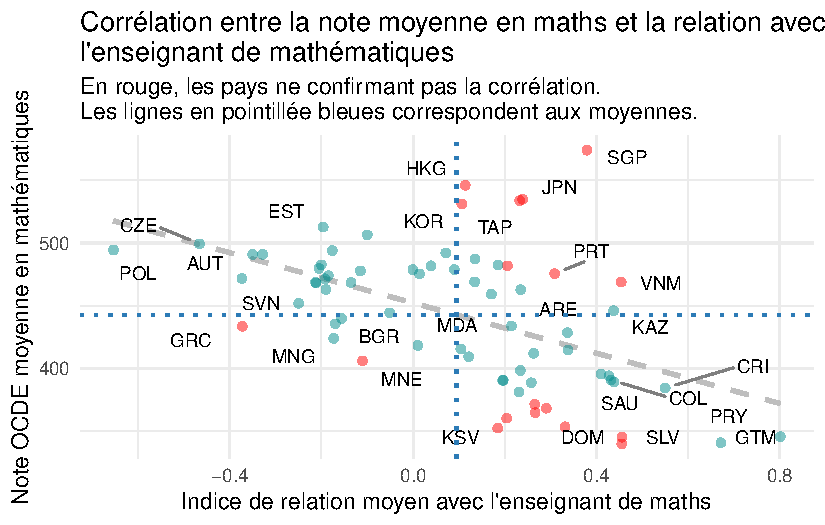
\includegraphics[keepaspectratio]{brouillon_rapport_files/figure-pdf/unnamed-chunk-20-1.pdf}}

Note de lecture : Le Kazakhstan (KAZ) a un niveau moyen en mathématiques
(445) équivalent à la moyenne des pays interrogés et un indice de REE
moyen plus positif qu'en moyenne (0.45).

Certains pays ne suivent pas cette corrélation négative, comme Singapour
(SGP) où la relation avec les enseignants de mathématiques est plus
postive de 0.4 point qu'en moyenne dans les pays de l'OCDE. De plus, le
niveau moyen en mathématiques y est le plus élevé. Le Guatemala (GTM)
confirme bien le lien de corrélation. Le niveau moyen en mathématiques
est largement en dessous de la moyenne, alors qu'on y retrouve la
meilleure REE moyenne.

\section{2.3 La REE et l'influence du statut
socio-économique}\label{la-ree-et-linfluence-du-statut-socio-uxe9conomique}

Si les notes et la REE sont corrélées, on peut tout de même s'interroger
sur l'influence du statut socio-économique des parents dans la relation
qu'entretient l'élève avec les enseignants. Autrement dit, les origines
sociales des élèves modifient-elles la manière dont ils intéragissent
avec le corps enseignant ?

\pandocbounded{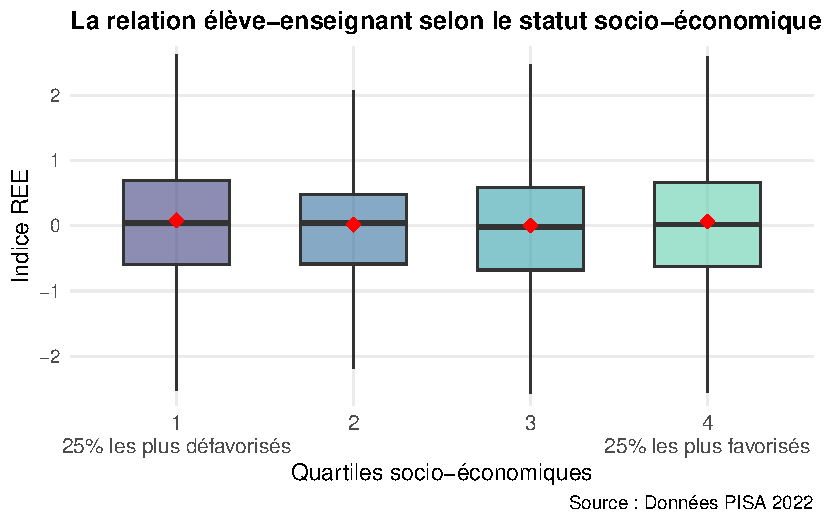
\includegraphics[keepaspectratio]{brouillon_rapport_files/figure-pdf/unnamed-chunk-21-1.pdf}}

Note de lecture : Les 50 \% d'élèves situés parmi les plus défavorisés
(quartile 1) rapportent des scores d'indice de REE compris entre environ
-0,7 et +0,8.

Note : L'indice REE est une variable composite : une valeur positive
indique une perception de la relation plus chaleureuse et soutenante que
la moyenne de l'OCDE, tandis qu'une valeur négative indique une relation
perçue comme plus distante ou moins aidante. Les losanges rouges
représentent la moyenne arithmétique de chaque groupe, tandis que la
ligne noire horizontale à l'intérieur de chaque boîte indique la médiane
(50 \% des élèves se situent au-dessus, 50 \% en dessous).

Le statut socio-économique des parents n'influence pas la qualité de la
relation entre élèves et enseignants, comme le montre le graphique
ci-dessus. Le vécu des élèves apparaît comme similaire quelques soient
les origines sociales. Les écarts inter-quartile sont très similaires
pour les quatres groupes socio-économiques, tout comme les moyennes et
les médianes.

\pandocbounded{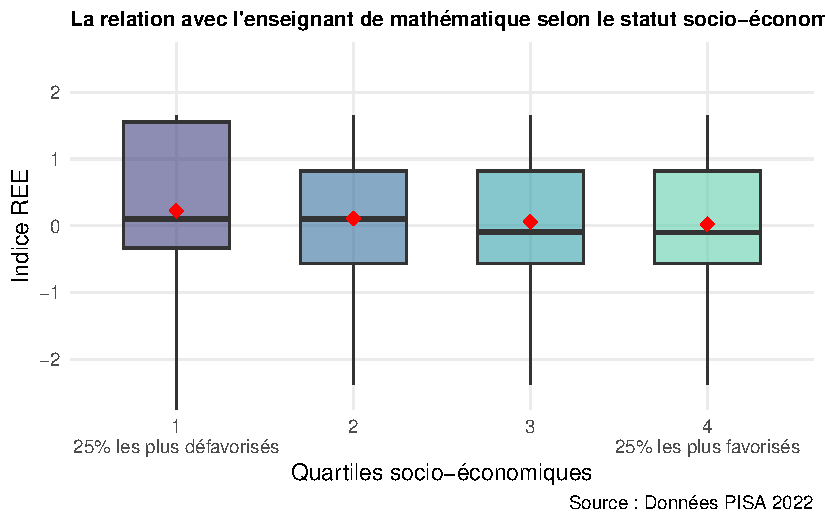
\includegraphics[keepaspectratio]{brouillon_rapport_files/figure-pdf/unnamed-chunk-22-1.pdf}}

Note de lecture : L'indice moyen de relation avec l'enseignant de
mathématiques pour les élèves appartenant au quart le plus défavorisé de
la population (quartile 1) se situe entre -0.3 et 1.5 pour la moitié
d'entre eux (dans la ``boîte'').

Cette dispersion autour de la qualité de la REE moyenne de l'OCDE change
lorsqu'on s'intéresse à la relation dans le cadre des mathématiques. Les
``boîtes'' des trois premiers quartiles sont plus hautes. Autrement dit,
l'écart interquartile est plus important pour les 25\% des élèves les
plus défavorisés, qui ont un vécu de la REE avec l'enseignant de
mathématiques plus hétérogène, allant de -0.3 à 1.5.

A l'échelle nationale, la REE et le statut socio-économique sont
corrélés négativement (-0.41). Lorsque dans un pays le statut
socio-économique moyen a tendance à être plus défavorisés, les élèves
observent en moyenne une meilleure relation avec leurs enseignants.
Inversement, dans les pays avec un statut socio-économique moyen
davatange favorisé, la REE est jugée plus négativement.

\begin{verbatim}
`geom_smooth()` using formula = 'y ~ x'
\end{verbatim}

\pandocbounded{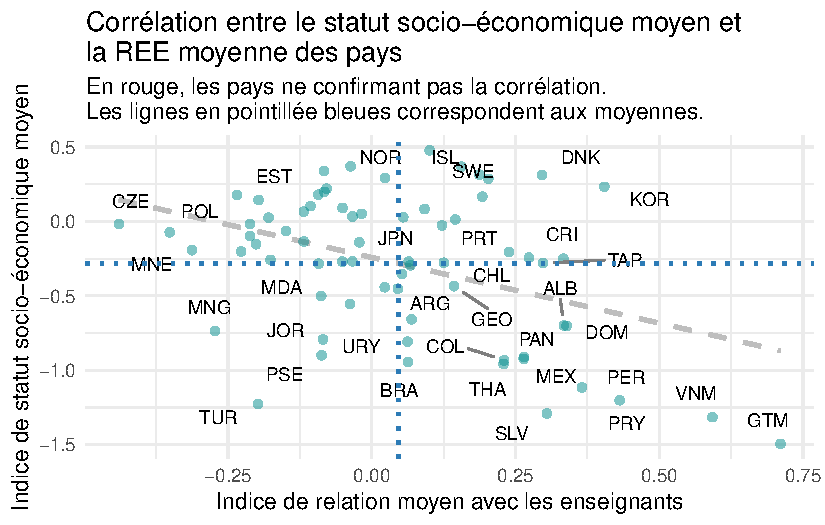
\includegraphics[keepaspectratio]{brouillon_rapport_files/figure-pdf/unnamed-chunk-24-1.pdf}}

Note de lecture : L'Albanie (ALB) a un indice socio-économique moyen
inférieur à la moyenne des pays interrogés (-0.75) ainsi qu'un indice de
REE moyen supérieur à la moyenne (0.3).

Le grapique illustre les différences de systèmes éducatifs entre les
différents pays interrogés. En effet, si à l'échelle individuelle on ne
constate pas de relation de corrélation significative entre les orgines
sociales et la qualité de la REE, en comparant les différents pays, on
peut conclure d'une influence. Cette corrélation négative oppose des
systèmes éducatifs tels que ceux du Vietnam (VNM) ou du Guatemala (GTM)
et ceux de la Pologne (POL) ou de la Tchéquie (CZE). D'un côté, on
retouve des pays dont les élèves ont des origines davantage défavorisées
et une REE plutôt positive, de l'autre côté des pays dont les élèves ont
un statut scoio-économique correspondant à la moyenne OCDE et une REE
jugée plus négativement qu'en moyenne au sein des pays de l'OCDE.

On peut en conclure que si, au niveau individuel, aucune corrélation
significative n'est observée, une corrélation modérée à forte apparaît
au niveau agrégé, c'est-à-dire au niveau des pays.

Cette différence suggère que le lien entre la qualité de la REE et le
statut social n'est pas individuel, mais une caractéristique systémique.
Cela révèle le fonctionnement des systèmes éducatifs et leur capacité à
créer une relation plus ou moins positive entre les élèves et les
enseignants.

\begin{tcolorbox}[enhanced jigsaw, bottomrule=.15mm, opacitybacktitle=0.6, left=2mm, colframe=quarto-callout-note-color-frame, title={Lien entre le statut socio-économique et le niveau scolaire des élèves}, breakable, coltitle=black, colbacktitle=quarto-callout-note-color!10!white, toptitle=1mm, rightrule=.15mm, opacityback=0, colback=white, leftrule=.75mm, toprule=.15mm, titlerule=0mm, arc=.35mm, bottomtitle=1mm]

Comme le présente de nombreuses études, le statut socio-économique des
parents est positivement corrélée avec le niveau scolaire. Il est même
possible de parler d'une relation de causalité. Avoir davantage de
ressources économiques et culturelles favorisent la réussite scolaire,
comme l'affirme l'OCDE dans son rapport sur l'enquête PISA 2022 : ``La
performance des élèves est associée au statut socio-économique, mais il
ne s'agit pas d'une relation immuable.''. En effet, ``En moyenne, dans
les pays de l'OCDE, les élèves socio-économiquement favorisé ont obtenu
93 points de plus en mathématiques que les élèves défavorisés.''

Cette relation entre l'origine sociale et le niveau scolaire explique
donc la présence de résultats similaires concernant la corrélation entre
la qualité de la REE et le niveau académique puis avec le statut
socio-économique.

\end{tcolorbox}

\section{2.4 REE et rapport aux
apprentissages}\label{ree-et-rapport-aux-apprentissages}

Au delà du niveau scolaire ou de statut socio-économique, l'appréciation
de l'élève concernant les matières étudiées peut partiellement expliquer
la qualité de la REE, notamment concernant la qualité de l'enseignement.

L'appréciation des mathématiques comme étant l'une des matières
préférées de l'élève est légérement corrélée avec la qualité de la
relation avec l'enseignement de cette matière. La corrélation s'élève à
environ 0.21 (p-value \textless{} 2.2e-16), ce qui permet de dire qu'il
y a bel et bien un lien entre ces deux éléments mais celui-ci reste
faible. Alors, aimer les maths ne suffit pas à expliquer une bonne
relation entre un élève et son enseignant de mathématiques.

La qualité perçue des cours de mathématiques est positivement corrélée
avec la qualité de la relation avec l'enseignant de mathématiques. En
effet, la corrélation est de 0.41 et est significative (p-value
\textless{} 2.2e-16). La qualité de la REE en maths est donc dépendante
de la qualité observée des cours de mathématiques au cours de l'année.

\chapter{3 Existe-t-il une relation entre la REE et le bien-être des
élèves dans le cadre scolaire
?}\label{existe-t-il-une-relation-entre-la-ree-et-le-bien-uxeatre-des-uxe9luxe8ves-dans-le-cadre-scolaire}

Nous étudierons ainsi dans quelle mesure cette relation d'enseignant à
élève peut impacter le bien-être de ces derniers.

Pour estimer le bien-être des élèves des pays de l'OCDE, nous utliserons
l'indice de bien-être ressenti durant les jours précédants. Cet indice
est construit grâce à la partie du questionnaire sur le bien-être.
L'indice s'affiche comme manquant lorsque l'élève n'a pas répondu
``Oui'' à la question ``La journée d'hier était-elle une journée comme
les autres ?''

Les indices suivants peuvent être étudiés afin d'élargir l'analyse et de
comprendre quels éléments influencent plus particulièrement les REE
comme le harcèlement, etc. D'autres variables et indices peuvent être
retenu pour expliquer la REE telles que l'indice d'anxiété concernant
les mathématiques, l'indice sur le sentiment d'appartenance à l'école ou
l'indice de harcèlement.

L'indice sur l'anxiété ressentie concernant les cours de mathématiques
permet d'approfondir l'analyse de l'indice de soutien de l'enseignant de
mathématiques (ANXMAT). Il est construit avec les réponses aux questions
concernant la crainte des difficultés en cours de mathématiques ou la
crainte de l'échec.

L'indice sur le sentiment d'appartenance, représente le sentiment
d'appartenance de l'élève à son école ainsi que l'existence de relations
avec d'autres à l'école (BELONG).

L'indice sur le harcèlement repose sur la fréquence de plusieurs signes
de harcèlement durant les 12 derniers mois, d'après les élèves
(BULLIED).

Enfin, on élabore alors une analyse en composantes principales sur nos
variables de bien-être, puis on trace le cercle des corrélation et
contributions des variables pour avoir une vue globale du problème,
c'est à dire pré-déterminer quels seront les différents liens, et ce sur
les 2 premiers axes de cette analyse en composante factorielle :

\pandocbounded{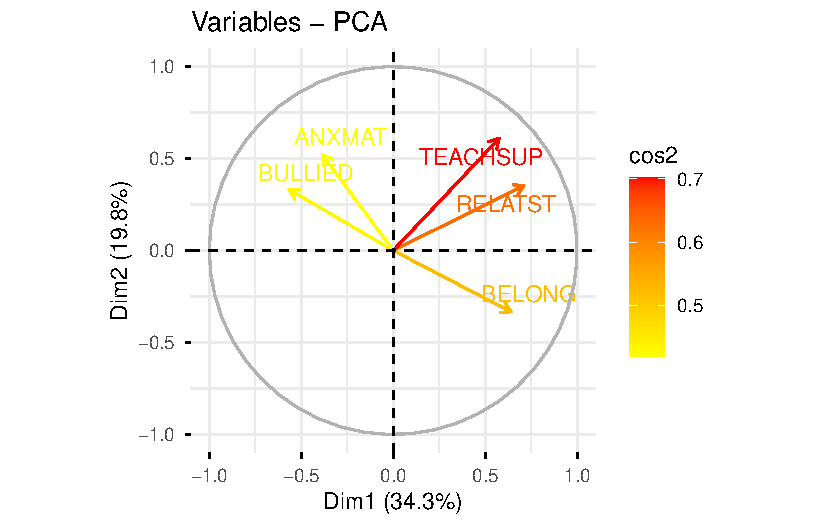
\includegraphics[keepaspectratio]{brouillon_rapport_files/figure-pdf/unnamed-chunk-26-1.pdf}}

TEACHSUP contribue grandement à l'analyse et se montre déjà presque en
lien avec RELATST. Ces deux variables représentent nos indices de
qualité REE, donc cela fait sens.

A contrario les indices ne semblent pas posséder de lien direct avec les
autres variables de bien-être sur ces premiers axes.

Voyons le en détail par la suite ;

\section{3.1 Existe t-il une relation entre la proximité de l'élève avec
l'enseignant et son bien-être ressenti à l'école
?}\label{existe-t-il-une-relation-entre-la-proximituxe9-de-luxe9luxe8ve-avec-lenseignant-et-son-bien-uxeatre-ressenti-uxe0-luxe9cole}

Ainsi, pour renforcer l'analyse, nous chercherons à déterminer aussi
quels sont les facteurs de bien-être.

\begin{Shaded}
\begin{Highlighting}[]
\NormalTok{vars }\OtherTok{\textless{}{-}}\NormalTok{ data\_etude }\SpecialCharTok{\%\textgreater{}\%}
  \FunctionTok{select}\NormalTok{(EXPWB, RELATST, TEACHSUP, ANXMAT, BELONG, BULLIED,)}
\end{Highlighting}
\end{Shaded}

\begin{Shaded}
\begin{Highlighting}[]
\NormalTok{vars }\SpecialCharTok{\%\textgreater{}\%}
  \FunctionTok{pivot\_longer}\NormalTok{(}\AttributeTok{cols =} \FunctionTok{everything}\NormalTok{()) }\SpecialCharTok{\%\textgreater{}\%}
  \FunctionTok{ggplot}\NormalTok{(}\FunctionTok{aes}\NormalTok{(}\AttributeTok{x =}\NormalTok{ value)) }\SpecialCharTok{+}
  \FunctionTok{geom\_histogram}\NormalTok{(}\AttributeTok{bins =} \DecValTok{30}\NormalTok{, }\AttributeTok{fill =} \StringTok{"steelblue"}\NormalTok{, }\AttributeTok{color =} \StringTok{"white"}\NormalTok{) }\SpecialCharTok{+}
  \FunctionTok{facet\_wrap}\NormalTok{(}\SpecialCharTok{\textasciitilde{}}\NormalTok{name, }\AttributeTok{scales =} \StringTok{"free"}\NormalTok{) }\SpecialCharTok{+}
  \FunctionTok{theme\_minimal}\NormalTok{()}
\end{Highlighting}
\end{Shaded}

\pandocbounded{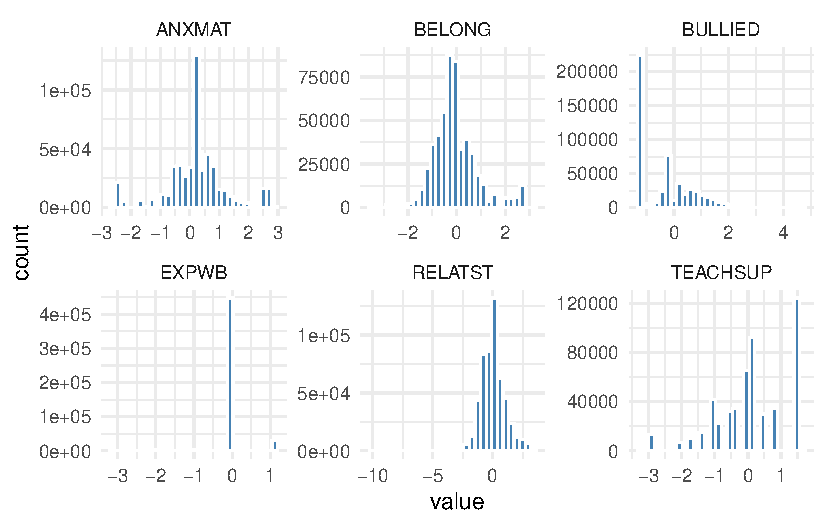
\includegraphics[keepaspectratio]{brouillon_rapport_files/figure-pdf/unnamed-chunk-28-1.pdf}}

On note ici que les indices sont centrés autour de 0, ils ont été
normalisés, ce qui facilite l'étude. De Plus on note que les dispersions
sont plutôt symétrique à l'exception du harcelèment.

\begin{Shaded}
\begin{Highlighting}[]
\NormalTok{cor\_matrix }\OtherTok{\textless{}{-}} \FunctionTok{cor}\NormalTok{(vars)}
\FunctionTok{corrplot}\NormalTok{(}
\NormalTok{  cor\_matrix,}
  \AttributeTok{method =} \StringTok{"color"}\NormalTok{,}
  \AttributeTok{type =} \StringTok{"upper"}\NormalTok{,}
  \AttributeTok{col =} \FunctionTok{colorRampPalette}\NormalTok{(}\FunctionTok{c}\NormalTok{(}\StringTok{"\#2c7bb6"}\NormalTok{, }\StringTok{"white"}\NormalTok{, }\StringTok{"\#d7191c"}\NormalTok{))(}\DecValTok{200}\NormalTok{),}
  \AttributeTok{tl.col =} \StringTok{"black"}\NormalTok{,}
  \AttributeTok{tl.srt =} \DecValTok{45}\NormalTok{,}
  \AttributeTok{addCoef.col =} \StringTok{"black"}\NormalTok{,}
  \AttributeTok{number.cex =} \FloatTok{0.7}\NormalTok{,}
  \AttributeTok{diag =} \ConstantTok{FALSE}
\NormalTok{)}
\end{Highlighting}
\end{Shaded}

\pandocbounded{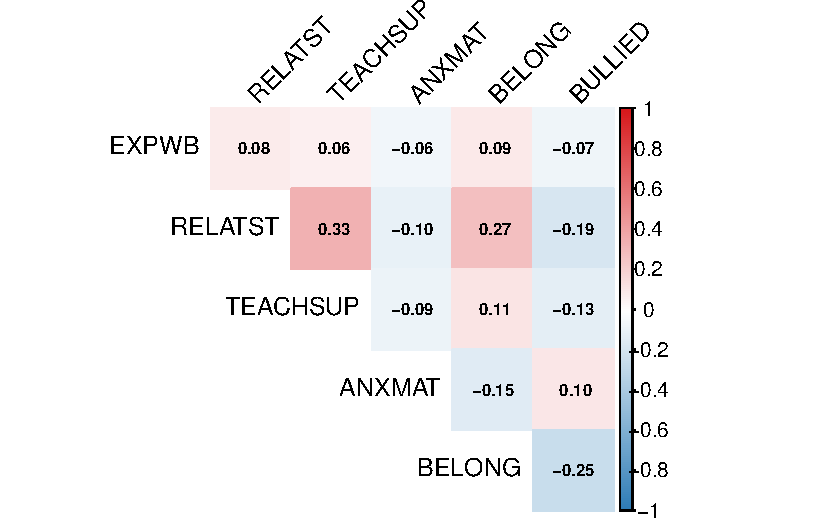
\includegraphics[keepaspectratio]{brouillon_rapport_files/figure-pdf/unnamed-chunk-29-1.pdf}}

\begin{verbatim}
`geom_smooth()` using formula = 'y ~ x'
\end{verbatim}

\pandocbounded{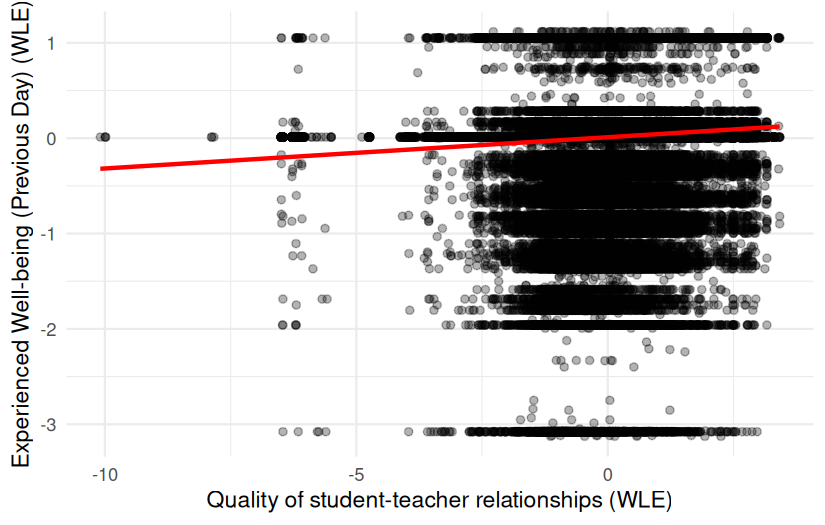
\includegraphics[keepaspectratio]{brouillon_rapport_files/figure-pdf/unnamed-chunk-30-1.png}}

En regardant le nuage de point entre notre premier indice et le
bien-être, on souligne que les individus ne semblent pas montrer une
dépendance ces variables. De plus la matrice de corrélation nous permet
de déterminer que la relation entre les différents indices de REE et le
bien-être semble faible (0.21 pour EXPWP avec RELATST). Cela dit, elle
n'est pas invisible.

\begin{verbatim}

Call:
lm(formula = EXPWB ~ RELATST + TEACHSUP + ANXMAT + BELONG + BULLIED, 
    data = vars)

Residuals:
    Min      1Q  Median      3Q     Max 
-3.2699 -0.0353  0.0000  0.0413  1.2443 

Coefficients:
              Estimate Std. Error t value Pr(>|t|)    
(Intercept)  0.0100890  0.0005917   17.05   <2e-16 ***
RELATST      0.0171971  0.0005993   28.70   <2e-16 ***
TEACHSUP     0.0116330  0.0005394   21.57   <2e-16 ***
ANXMAT      -0.0166497  0.0005373  -30.99   <2e-16 ***
BELONG       0.0266097  0.0006301   42.23   <2e-16 ***
BULLIED     -0.0163631  0.0005736  -28.53   <2e-16 ***
---
Signif. codes:  0 '***' 0.001 '**' 0.01 '*' 0.05 '.' 0.1 ' ' 1

Residual standard error: 0.3977 on 527314 degrees of freedom
Multiple R-squared:  0.01692,   Adjusted R-squared:  0.01691 
F-statistic:  1815 on 5 and 527314 DF,  p-value: < 2.2e-16
\end{verbatim}

En élaborant un modèle linéaire à l'aide de nos indicateurs, on voit que
la p-value de chacun d'entre eux est très faible (vis-à-vis du test de
significativité des coefficients). On en déduit qu'il n'y a visiblement
pas de relation entre la REE et le bien-être, de manière générale.

Nous nous proposons ainsi de ré-effectuer cette étude en la croisant
avec de nouvelles variables.

\section{3.2 L'impact de variables externes sur le lien entre REE et
bien-être}\label{limpact-de-variables-externes-sur-le-lien-entre-ree-et-bien-uxeatre}

\subsection{3.2.1 Dans quelles mesures le statut socio-économique des
élèves influence leur bien-être, la REE, et donc l'impact du bien-être
sur la REE
?}\label{dans-quelles-mesures-le-statut-socio-uxe9conomique-des-uxe9luxe8ves-influence-leur-bien-uxeatre-la-ree-et-donc-limpact-du-bien-uxeatre-sur-la-ree}

Utilisons pour ce faire la variable ESCS.

Dans les enquêtes PISA, l'ESCS (indice de statut économique, social et
culturel) est un indicateur qui mesure le milieu socio-économique des
élèves à partir du niveau d'éducation et de la profession des parents
ainsi que des ressources du foyer (comme les livres ou l'accès à un
ordinateur).

\begin{verbatim}

 Faible Moyenne  Élevée 
 174026  174009  179285 
\end{verbatim}

Par souci de compléxité, on décide de scinder l'indice de catégorie
socio professionnelle en variable qualitative. En utilisant 2 tertilles,
on obtient directement tous les individus avec un indice de CSP faisant
partis des 33\% les plus faibles, ceux faisant partis des 66\% les plus
faibles ET des 66\% les plus élevés, et faisant partis des 33\% les plus
élevés. On distingue alors 3 classes, les CSP faibles, moyennes, et
élevées.

On remarque la robustesse statistique de notre jeu de données avec des
effectifs très similaires dans chaque classe.

\pandocbounded{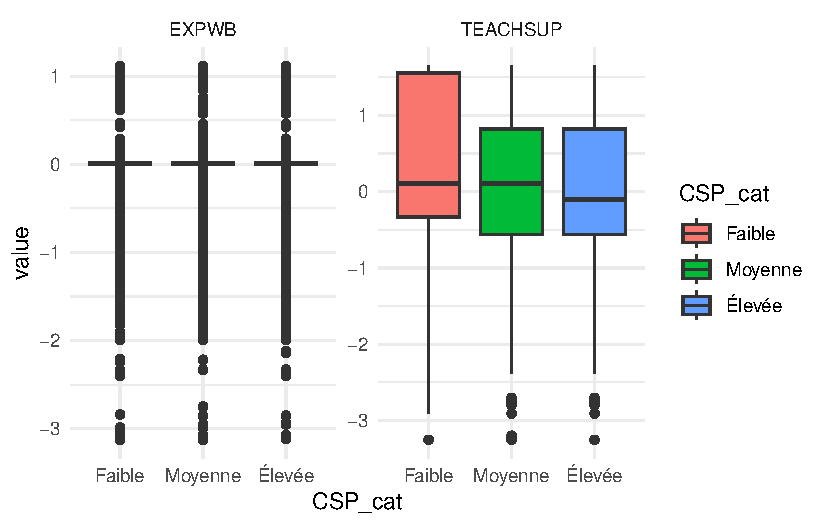
\includegraphics[keepaspectratio]{brouillon_rapport_files/figure-pdf/unnamed-chunk-35-1.pdf}}

Comparons nos classes selon le bien-être, et la REE, de leurs individus.
La CSP semble peu agir sur cela. Toutefois on remarque que les élèves
issus de parents avec des catégories socio professionnelles élevées
montrent une moins bonne relation entre élève et enseignant.

\begin{verbatim}
`geom_smooth()` using formula = 'y ~ x'
\end{verbatim}

\pandocbounded{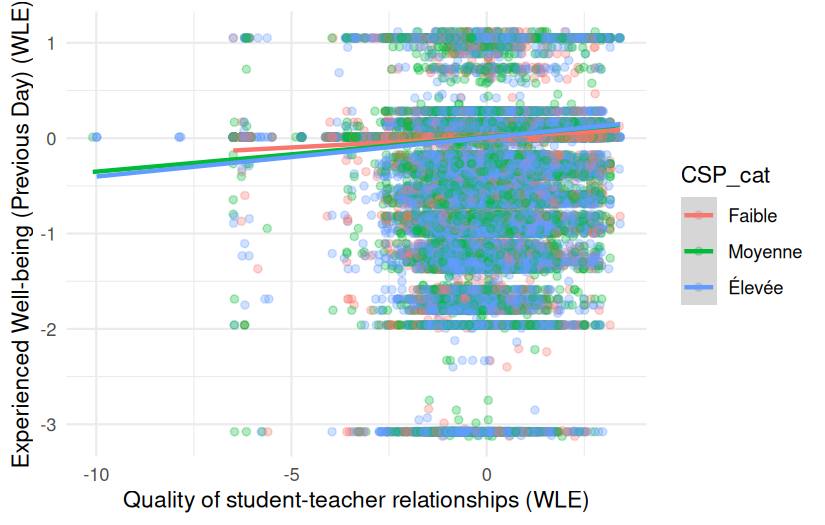
\includegraphics[keepaspectratio]{brouillon_rapport_files/figure-pdf/unnamed-chunk-36-1.png}}

On trace sur le même nuage de points tous les individus, différenciés
par leur CSP. On note que la pente, ou coefficient directeur, de la
regression (REE \textasciitilde{} Bien-être) est plus forte dans le cas
des catégories socio professionnelles élevées. Même si la différence est
faible, les élèves de haute CSP sont plus touchés par les REE, c'est à
dire que leur bien-être en dépend plus. Cela va dans le sens de notre
analyse précédente ; si les élèves montrent être plus affectés par la
REE, il fait sens que la REE ne soit pas ``moyenne'' et inéxistante,
mais bien forte ou faible (faible dans ce cas-ci).

Construisons maintenant un modèle comportant les CSP pour voir si
celles-ci se montrent impactantes ;

\begin{verbatim}

Call:
lm(formula = EXPWB ~ RELATST * CSP_cat + TEACHSUP + ANXMAT + 
    BELONG + BULLIED, data = vars_csp)

Residuals:
    Min      1Q  Median      3Q     Max 
-3.2660 -0.0351  0.0000  0.0413  1.2822 

Coefficients:
                         Estimate Std. Error t value Pr(>|t|)    
(Intercept)             0.0155303  0.0010007  15.519   <2e-16 ***
RELATST                 0.0082437  0.0009498   8.680   <2e-16 ***
CSP_catMoyenne         -0.0028043  0.0013531  -2.072   0.0382 *  
CSP_catÉlevée          -0.0125893  0.0013559  -9.284   <2e-16 ***
TEACHSUP                0.0111451  0.0005408  20.607   <2e-16 ***
ANXMAT                 -0.0169641  0.0005399 -31.422   <2e-16 ***
BELONG                  0.0269023  0.0006330  42.497   <2e-16 ***
BULLIED                -0.0162859  0.0005736 -28.395   <2e-16 ***
RELATST:CSP_catMoyenne  0.0126039  0.0013506   9.332   <2e-16 ***
RELATST:CSP_catÉlevée   0.0150160  0.0013094  11.468   <2e-16 ***
---
Signif. codes:  0 '***' 0.001 '**' 0.01 '*' 0.05 '.' 0.1 ' ' 1

Residual standard error: 0.3976 on 527310 degrees of freedom
Multiple R-squared:  0.01736,   Adjusted R-squared:  0.01735 
F-statistic:  1035 on 9 and 527310 DF,  p-value: < 2.2e-16
\end{verbatim}

Finalement, les coefficients directeurs des différents milieux sociaux
sont faibles et ne permettent pas de conclure à une dépendance entre la
REE dans ces derniers et le bien-être.

D'ailleurs, ce résultat peut-être généralisé dans l'autre sens, ie : Le
bien-être dans chaque contexte socio-professionnel n'explique pas la
relation entre élève et enseignant.

Cela dit, l'indice ESCS est un indicateur synthétique du statut
socio-économique, il permet des comparaisons standardisées, mais cache
certaines différences spécifiques et repose sur des déclarations dites
``auto-rapportées'', ce qui nécessite plus de prudence dans
l'interprétation des résultats.

\subsection{3.2.2 Le sexe de l'élève peut-il modifier la relation entre
bien-être et REE
?}\label{le-sexe-de-luxe9luxe8ve-peut-il-modifier-la-relation-entre-bien-uxeatre-et-ree}

Si les catégories socio-professionnelles des parents de l'élève ne
semblent pas modifier le lien REE à bien-être, peut-être que le sexe le
pourra.

Ainsi l'objectif est d'identifier d'éventuelles inégalités ou
sensibilités spécifiques des élèves selon leur sexe auprès de
l'influence des REE sur leur bien-être.

\begin{verbatim}

 Femme  Homme 
262209 265074 
\end{verbatim}

Pour commencer, on vérifie que l'échantillon est bien représentatif ; Ce
dernier comporte 51\% de femmes pour 49\% d'hommes. Ce qui nous
conviendra pour l'étude.

\begin{verbatim}
# A tibble: 2 x 13
  sexe  EXPWB_mean EXPWB_sd RELATST_mean RELATST_sd TEACHSUP_mean TEACHSUP_sd
  <fct>      <dbl>    <dbl>        <dbl>      <dbl>         <dbl>       <dbl>
1 Femme   -0.00589    0.423       0.0603      0.973        0.112         1.10
2 Homme    0.0286     0.378       0.0205      1.04         0.0962        1.06
# i 6 more variables: ANXMAT_mean <dbl>, ANXMAT_sd <dbl>, BELONG_mean <dbl>,
#   BELONG_sd <dbl>, BULLIED_mean <dbl>, BULLIED_sd <dbl>
\end{verbatim}

\pandocbounded{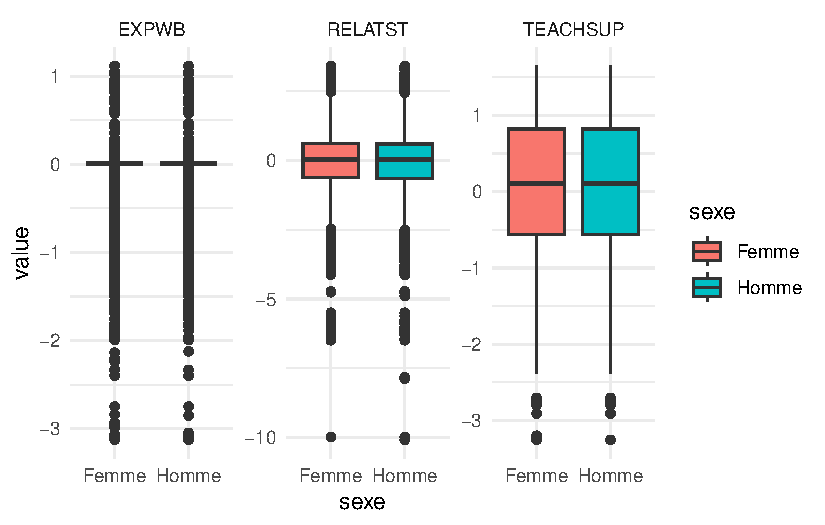
\includegraphics[keepaspectratio]{brouillon_rapport_files/figure-pdf/unnamed-chunk-41-1.pdf}}

On remarque par des statistiques descriptives simples et des
représentations visuelles que les hommes montrent un bien-être plus
élevé que les femmes. En revanche la relation entre élèves et enseignant
semble être en moyenne de meilleure qualité en ce qui concerne les
femmes. Par ailleurs, la relation entre les hommes et leur enseignant
est la même que celle des femmes avec leur enseignant.

\begin{verbatim}
`geom_smooth()` using formula = 'y ~ x'
\end{verbatim}

\pandocbounded{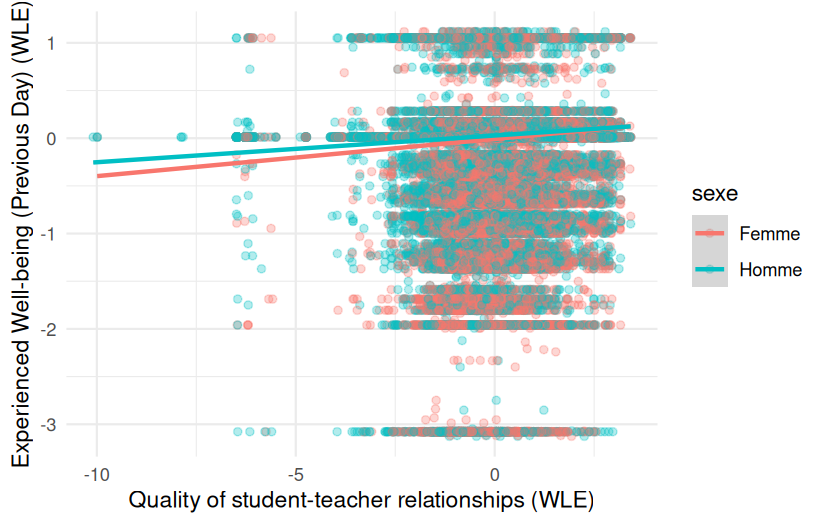
\includegraphics[keepaspectratio]{brouillon_rapport_files/figure-pdf/unnamed-chunk-42-1.png}}

Le graphique ci-dessus indique que la relation entre élève et enseignant
impacte le bien-être de manière plus imortante chez les femmes. Les
hommes n'en sont pas dépouvus non plus.

Etudions le lien directement avec un coefficient de correlation
différencié par sexe ;

\begin{verbatim}
# A tibble: 2 x 2
  sexe  correlation
  <fct>       <dbl>
1 Femme      0.0897
2 Homme      0.0768
\end{verbatim}

Les correlations entre REE et bien-être restent faibles, mais sont
existantes tout de même. Une part du bien être s'explique donc par la
REE, et ce, plus fortement chez les femmes.

On se propose maintenant de créer le modèle linéaire expliquant le
bien-être par la REE et le sexe de l'élève.

\begin{verbatim}

Call:
lm(formula = EXPWB ~ RELATST * sexe + TEACHSUP + ANXMAT + BELONG + 
    BULLIED, data = vars_sex)

Residuals:
    Min      1Q  Median      3Q     Max 
-3.2581 -0.0379  0.0015  0.0434  1.2803 

Coefficients:
                    Estimate Std. Error t value Pr(>|t|)    
(Intercept)       -0.0058465  0.0008380  -6.976 3.03e-12 ***
RELATST            0.0223278  0.0008431  26.483  < 2e-16 ***
sexeHomme          0.0297616  0.0011129  26.742  < 2e-16 ***
TEACHSUP           0.0115711  0.0005393  21.456  < 2e-16 ***
ANXMAT            -0.0145610  0.0005425 -26.842  < 2e-16 ***
BELONG             0.0252113  0.0006316  39.916  < 2e-16 ***
BULLIED           -0.0174596  0.0005747 -30.379  < 2e-16 ***
RELATST:sexeHomme -0.0083460  0.0010922  -7.641 2.16e-14 ***
---
Signif. codes:  0 '***' 0.001 '**' 0.01 '*' 0.05 '.' 0.1 ' ' 1

Residual standard error: 0.3973 on 527275 degrees of freedom
Multiple R-squared:  0.01832,   Adjusted R-squared:  0.01831 
F-statistic:  1406 on 7 and 527275 DF,  p-value: < 2.2e-16
\end{verbatim}

D'abord, on remarque que les coefficients directeurs concernant les
modalités de sexe sont les plus élevées du modèle. De plus, le R² de ce
modèle est légèrement supérieur aux deux précédents. (0.1116
\textgreater{} 0.103 \textgreater{} 0.098)

Dans notre étude, nous affirmons donc que le sexe doit être plus pris en
compte que la catégorie socio-professionnelle dans l'analyse du
bien-être selon la REE.

\subsection{3.2.3 En quoi l'appartenance où non d'un pays à l'OCDE
influence ses élèves dans leur bien-être vis-à-vis de leur relation avec
leur enseignant
?}\label{en-quoi-lappartenance-ouxf9-non-dun-pays-uxe0-locde-influence-ses-uxe9luxe8ves-dans-leur-bien-uxeatre-vis-uxe0-vis-de-leur-relation-avec-leur-enseignant}

L'OCDE (Organisation de Coopération et de Développement Économiques) est
une organisation internationale regroupant principalement des pays
développés. Elle promouvoit des politiques publiques favorisant le
bien-être social et l'amélioration des systèmes éducatifs. Dans le cadre
des enquêtes PISA, elle s'avère jouer un rôle central, permettant de
déterminer si un élève étudié inscrit son parcours scolaire dans un
contexte mélioratif ou non.

\begin{verbatim}

Non-OCDE     OCDE 
  261487   265833 
\end{verbatim}

A l'inverse des variables externes précédentes, notre échantillon
possède ici beaucoup plus d'élèves appartenant à une des modalités
qu'une autre. En effet seulement 36\% des élèves de l'échantillon
n'appartiennent pas à un pays compris dans l'OCDE, contre 64\% qui y
appartiennent.

\begin{verbatim}
# A tibble: 2 x 7
  OCDE_cat     EXPWB  RELATST TEACHSUP ANXMAT   BELONG BULLIED
  <fct>        <dbl>    <dbl>    <dbl>  <dbl>    <dbl>   <dbl>
1 Non-OCDE  0.0239   0.0809     0.235   0.261 -0.127    -0.280
2 OCDE     -0.000808 0.000318  -0.0252  0.189  0.00786  -0.304
\end{verbatim}

\pandocbounded{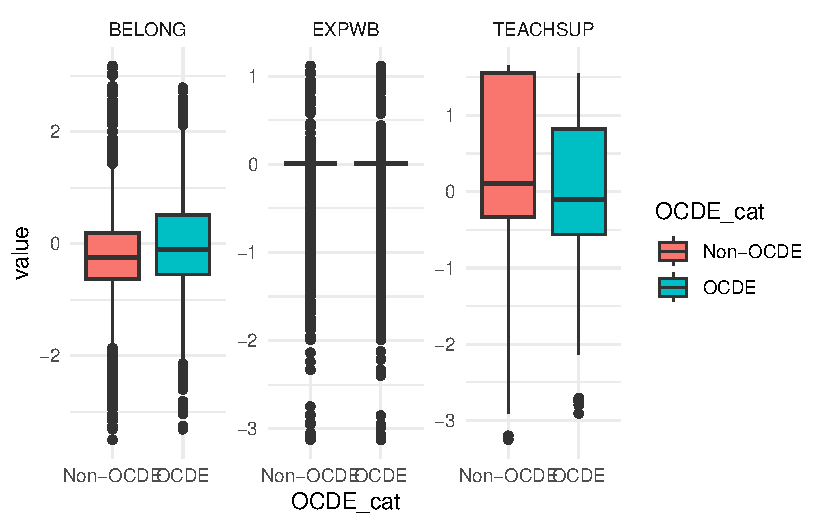
\includegraphics[keepaspectratio]{brouillon_rapport_files/figure-pdf/unnamed-chunk-48-1.pdf}}

Tout d'abord, les élèves de l'OCDE semblent moins ressentir de
bien-être, et beaucoup moins de relation avec les enseignants, si l'on
s'en tient à l'indice TEACHSUP plutôt qu'à RELATST. Par ailleurs, les
élèves de l'OCDE semblent avoir un sentiment d'appartenance plus fort à
leur école.

Etudions tout cela plus en profondeur ;

\begin{verbatim}
`geom_smooth()` using formula = 'y ~ x'
\end{verbatim}

\pandocbounded{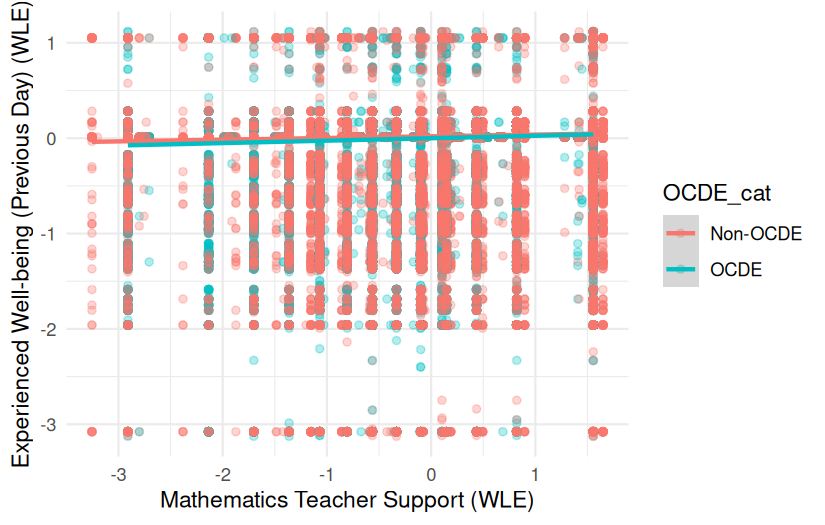
\includegraphics[keepaspectratio]{brouillon_rapport_files/figure-pdf/unnamed-chunk-49-1.png}}

\begin{verbatim}
`geom_smooth()` using formula = 'y ~ x'
\end{verbatim}

\pandocbounded{\includegraphics[keepaspectratio]{brouillon_rapport_files/figure-pdf/unnamed-chunk-50-1.pdf}}

Pour plus de précisions et comme l'indice TEACHSUP se montre être plus
intéressant dans ce cas là. On étudie les deux indices de REE établis
par PISA.

De prime abord, notons que dans chaque cas, la REE s'améliore avec le
bien-être, et la non-appartenance à l'OCDE. En revanche, on voit que le
coefficient directeur de la variable explicative est plus fort pour
RELATST. A noter que cet indicateur concerne moins les mathématiques que
l'autre. On peut alors expliquer le phénomène de la manière suivante ;
Les élèves ont un bien-être plus grandissant et lié à la relation avec
leur professeur lorsque ceux-ci étudient moins les mathématiques.

En outre on construit le modèle correpondant pour vérifier les
hypothèses émises.

\begin{verbatim}

Call:
lm(formula = EXPWB ~ RELATST * OCDE_cat + TEACHSUP + ANXMAT + 
    BELONG + BULLIED, data = vars_oecd)

Residuals:
    Min      1Q  Median      3Q     Max 
-3.2681 -0.0372  0.0005  0.0421  1.3020 

Coefficients:
                       Estimate Std. Error t value Pr(>|t|)    
(Intercept)           0.0241888  0.0008237   29.37   <2e-16 ***
RELATST               0.0096253  0.0007850   12.26   <2e-16 ***
OCDE_catOCDE         -0.0267566  0.0011087  -24.13   <2e-16 ***
TEACHSUP              0.0098266  0.0005432   18.09   <2e-16 ***
ANXMAT               -0.0170395  0.0005373  -31.71   <2e-16 ***
BELONG                0.0276771  0.0006318   43.80   <2e-16 ***
BULLIED              -0.0164646  0.0005732  -28.72   <2e-16 ***
RELATST:OCDE_catOCDE  0.0155380  0.0010920   14.23   <2e-16 ***
---
Signif. codes:  0 '***' 0.001 '**' 0.01 '*' 0.05 '.' 0.1 ' ' 1

Residual standard error: 0.3974 on 527312 degrees of freedom
Multiple R-squared:  0.01833,   Adjusted R-squared:  0.01832 
F-statistic:  1407 on 7 and 527312 DF,  p-value: < 2.2e-16
\end{verbatim}

Les coefficients directeurs associés à l'appartenance ou non à l'OCDE
sont les plus importants du modèle. Le lien est toujours faible. Cela
dit, nous pouvons dire que le bien-être est déterminé par la REE, de
manière plus marquée hors de l'OCDE. De plus cet appartenance ou non à
cette organisation est la variable la plus efficace pour caractériser le
bien-être selon la REE, en comparant aux autres variables externes. On
utilise le critère du R² pour justifier cela (0.1122 \textgreater{}
0.1116 \textgreater{} 0.103 \textgreater{} 0.098).

Toutefois, cette variable externe est aussi une varible binaire et donc
très simplificatrice qui ne montre pas précisément quels sont les état
de développement des pays étudiés.

Cette classification peut ainsi cacher des différences importantes entre
pays et ne permet pas de montrer la potentielle influence réelle des
systèmes éducatifs sur la relation élève-enseignant et par conséquent le
bien-être.

\section{3.3 Qu'en est-il réellement de l'impact de la relation entre
élève et enseignant sur le bien-être de l'élève
?}\label{quen-est-il-ruxe9ellement-de-limpact-de-la-relation-entre-uxe9luxe8ve-et-enseignant-sur-le-bien-uxeatre-de-luxe9luxe8ve}

L'objectif de cette étude était d'analyser l'influence de la relation
élève-enseignant sur le bien-être des élèves, en supposant l'existence
d'un lien positif, potentiellement renforcé ou modulé par des variables
comme le statut socio-économique, le sexe ou l'appartenance à l'OCDE.

Toutefois, les résultats obtenus nuancent ces attentes : la relation
élève-enseignant n'apparaît que faiblement liée au bien-être, et
l'introduction de variables complémentaires n'a pas permis d'en
améliorer significativement l'explication.

Ces résultats suggèrent que le bien-être des élèves repose sur des
facteurs plus complexes que ceux étudiés ici et invitent à adopter une
approche plus globale de cette problématique.

\chapter{Annexe}\label{annexe}

\subsection{Méthodologie de construction des
indices}\label{muxe9thodologie-de-construction-des-indices}

L'indice de qualité des relations entre élèves et enseignants (RELATST)
permet de savoir lorsque l'élève fait l'état d'une meilleure relation
que l'état moyen des pays de l'OCDE. Cet indice est réalisé à partir des
réponses de la question 267. Le second indice concerne quant à lui la
question 270 sur le soutien du professeur de mathématiques (TEACHSUP).
Il fonctionne de la même manière que le premier indice, plus il est
positif, plus l'élève affirme bénéficier d'un soutien de son enseignant
plus important qu'en moyenne.

Le statut social et culturel (ESCS) est un indice composite complexe
issus du questionnaire élève. Il réutilise d'autres indices que sont le
statut professionnel le plus élevé des parents (HISEI), le niveau
d'éducation le plus élevé des parents (PAREDINT) et les biens possédés
par le foyer (HOMEPOS). Le statut socio-économique sera donc considéré à
partir du statut professionnel, du niveau d'éducation et du revenu du
foyer. Lorsque l'un des trois indices utilisés affiche une valeur
manquante, celle-ci a été remplacé par une prédiction. Dans le cas où
plusieurs données étaient manquantes, la valeur NA a été retenue. Les
indices ont été standardisés afin de permettre une contribution égale de
chaque pays de l'OCDE. La moyenne de l'indice ESCS est à 0 tandis que
sont écart-type est à 1.

Pour les variables concernant les notes des élèves lors des épreuves
PISA en mathématiques, science et lecture, l'étude se basera sur les
moyennes des 10 valeurs plausibles estimées par l'OCDE (de type
``PV\ldots{}'') afin de standardiser les résultats obtenus par les
élèves dans chaque domaines. Afin d'étudier les REE, notre étude
utilisera 3 notes par élèves, et notamment celle en mathématiques,ainsi
qu'une moyenne de ces notes.

Pour estimer le bien-être des élèves des pays de l'OCDE, nous utliserons
l'indice de bien-être ressenti durant les jours précédants (EXPWB). Cet
indice est construit à partir de la question WB178, du questionnaire sur
le bien-être. L'indice s'affiche comme manquant lorsque l'élève n'a pas
répondu ``Oui'' à la question ``La journée d'hier était-elle une journée
comme les autres ?''

L'indice sur l'anxiété ressentie concernant les cours de mathématiques
(ANXMAT) permet d'approfondir l'analyse de l'indice de soutien de
l'enseignant de mathématiques. Il est construit à partir de la question
ST292 concernant la crainte des difficultés en cours de mathématiques ou
la crainte de l'échec. (voir PISA 2021 pour la méthodologie)

L'indice sur le sentiment d'appartenance (BELONG), représente le
sentiment d'appartenance de l'élève à son école ainsi que l'existence de
relations avec d'autres à l'école (ST034). (voir PISA 2018 pour
méthodologie)

L'indice sur le harcèlement (BULLIED) repose sur la fréquence de
plusieurs signes de harcèlement durant les 12 derniers mois (ST038),
d'après les élèves. (voir PISA 2018 pour méthodologie)

L'indice sur l'utilisation des technologies de l'information et de la
communication (TIC) en rapport avec la matière enseignée (ICTSUBJ) est
construit à partir de la question IC173. Cette question concerne la
fréquence d'utilisation des TIC.

Lien pour plus de détails méthodologiques concernant les indices
construits par l'OCDE :
https://www.oecd.org/content/dam/oecd/en/publications/reports/2024/03/pisa-2022-technical-report\_599753f0/01820d6d-en.pdf




\end{document}
